\documentclass[tog]{acmsiggraph}
\graphicspath{{./images/}}
\usepackage{gensymb}
\usepackage[ngerman]{babel}
\usepackage[utf8]{inputenc}
\usepackage[T1]{fontenc}
\usepackage{hyperref}
\usepackage{listings}
\usepackage{amsmath}
\newcommand{\code}[1]{\texttt{#1}}
%%% Make the ``BibTeX'' word pretty...
\def\BibTeX{{\rm B\kern-.05em{\sc i\kern-.025em b}\kern-.08em
    T\kern-.1667em\lower.7ex\hbox{E}\kern-.125emX}}

%%% Used by the ``review'' variation; the online ID will be printed on 
%%% every page of the content.

\TOGonlineid{00001}

%%% Used by the ``preprint'' variation.

\TOGvolume{0}
\TOGnumber{0}

\title{Übung 1 - Computergrafik-I, WS 2015/16}
\author{Christoph Stumpe, Fabian Wendland, Martin Zier\\Beuth Hochschule für Technik Berlin}
\pdfauthor{Martin Zier, s59330}
\date{25. Oktober 2015}

\keywords{Matrizen, Mathematik, Java Übung}

\begin{document}

\teaser{
   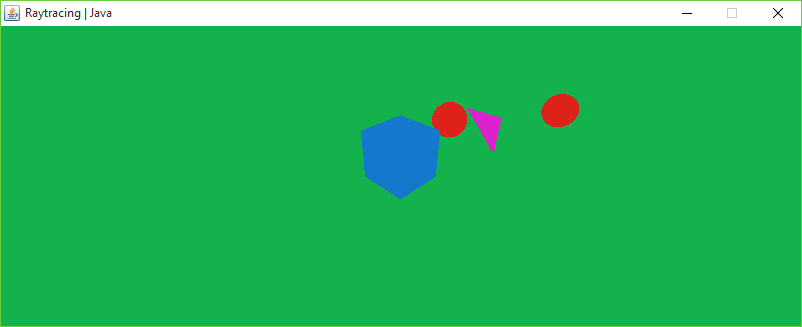
\includegraphics[height=2in]{02_tracing-frame.png}
   \caption{Übungsinhalt der zweiten Aufgabe}
   }
\maketitle

\tableofcontents

\section{Einführung}
Die Aufgaben der zweiten Übung umfassen die ersten Darstellungen von Bildern und rendern von simplen Objekten, darunter Ebenen, Kugeln, Dreiecke und eine Axis-Aligned Box. Dabei wird das gesamte Grundprogramm des Raytracers geschrieben und auf die Vektorbibliothek aus der ersten Übung zurückgegriffen.

\section{Aufgabenstellung}

Alle dargestellten Aufgaben beziehen sich auf die Implementierung mit Java sofern nicht anders gekennzeichnet.

\subsection{Strahlengenerierung}

Das Objekt \code{Ray} repräsentiert einen ausgesendeten Strahl, der von der gewählten Kamera ausgeht. Es kann daraus erechnet werden, an welchem Punkt im Raum sich der Strahl befindet für ein bestimmtes \code{t} oder wie groß das \code{t} an einem bestimmten Punkt ist.

\subsection{Kameras}

Es soll eine abstrakte Klasse \code{Camera} erstellt werden, die bereits Informationen für eine \code{OrthographicCamera} und eine \code{PerspectiveCamera} beinhaltet. Diese zwei erbenden Klassen erweitern die Superklasse um die benötigten Klassenattribute und können \code{Rays} generieren.

\subsection{Farben}

Die Klasse \code{Color} soll eine RGB-Farbe mit separaten \code{double}-Werten repräsentieren, wobei jeder Farbkanal \code{>= 0} sein muss. Diese Farben können miteinander addiert, subtrahiert und multipliziert werden, welches für spätere Übungen verwendet wird.

\subsection{Geometrie}

Für die Geometrie wird eine Superklasse \code{Geometry} erstellt, aus der \code{Plane}, \code{AxisAlignedBox}, \code{Triangle} und \code{Sphere} erben. Die Geometrie-Objekte können ein neues, separates \code{Hit}-Objekt zurückliefern, wenn ein ausgesenderter \code{Ray} auf das Objekt trifft.

\subsection{Welt}

Eine neue Klasse \code{World} beinhaltet alle geometrischen Informationen und eine Hintergrundfarbe. Diese Hintergrundfarbe wird benutzt, wenn ein Strahl kein Objekt trifft.

\subsection{Raytracer}

Das Herzstück der Anwendung ist der \code{Raytracer}, der über alle Pixel der zu renderenden Ebene iteriert und die Berechnung der Farbwerte einer Szenerie durchführt.

\subsection{OpenCL Implementierung}

In dem vorherigen Papier zur Übung 1 wurde eine Python-Implementierung vorgeschlagen. Unsere Gruppe hat sich danach entschieden den Raytracer in OpenCL zu implementieren. Die Vorbereitungen für ein Rendering in OpenCL werden bereits getroffen.

\section{Lösungsstrategien}

Da die Komplexität des Problems nur sehr klein ist und die benötigte Implementierung mehr eine Fleißaufgabe (oder Tippaufgabe) ist, hat einer die Tracer-Applikation geschrieben, einer geprüft und der letzte bereits einen C++-Host und OpenCL-Kernel angelegt.

\section{Implementierung und Bearbeitungszeit}

Da es bereits eine sehr strikte systematische Planung vorgegeben wurde, musste keine große Vorplanung der Implementierung getroffen werden.

\subsection{Strahlengenerierung}

Die Strahlengenerierung erwies sich als sehr einfach.

\textbf{Bearbeitungszeit:} 0,5 - 1 Stunde

\subsection{Kameras}

Durch unentdeckte Fehler der Vektorenbibliothek hat das Debugging der Kameras viel Zeit benötigt. Diese Fehler hätten mit intensiveren Prüfungen im Vorfeld der ersten Übung vermieden werden können.

\textbf{Bearbeitungszeit:} 2 - 3 Stunden

\subsection{Farben}

Die Farbberechnung ist mit unter den einfachsten Aufgaben der Übung gewesen.

\textbf{Bearbeitungszeit:} 1 Stunde

\subsection{Geometrie}

Da die Geometrien umfangreich sind und sich vor allem bei der Axis-Aligned Box einige Probleme aufgetreten sind, erwies sich die Bearbeitung der Geometrien weitaus länger als gedacht. Durch den Hinweis der Gleitkomma-Fehlerberechnung wurden die Probleme jedoch gelöst und die Fehlerbilder wurden aufgehoben.

\textbf{Bearbeitungszeit:} 4 Stunden

\subsection{Welt}

Auch die Klasse \code{World} ist ohne versteckte Probleme zu bearbeiten gewesen. Durch eine \code{ArrayList} gibt es eine erweiterbare Liste und die Verwendung von einer solchen Collection ist für den Moment vollkommen ausreichend für die Performance.

\textbf{Bearbeitungszeit:} 30 Minuten

\subsection{Raytracer}

Der Raytracer wurde im Verlauf immer wieder angepasst, da hauptsächlich die dynamische Weltveränderung Anfangs nicht möglich war.

\subsection{OpenCL Implementierung}

Die OpenCL Implementierung ist noch in Bearbeitung - die hauptsächlichen Problematiken sind folgende:

\begin{itemize}

\item \textbf{Datentransport von Host zu Kernel:} Es stellt sich heraus, dass es nur sehr schwierig ist, Daten vollständig und funktionell zu übertragen, so dass der OpenCL Kernel sinnvoll diese Daten weiter verarbeiten kann. Das Problem ist bis jetzt nicht gelöst.

\item \textbf{Interoperation OpenGL \& OpenCL:} Uns scheint es sinnvoll ein Fenster mit OpenGL darzustellen - dadurch wird auch die Grafikhardware optimal ausgenutzt und durch viele built-in Features von SDL (Simple DirectMedia Layer) ist die Bilddarstellung einfach und möglichst effizient.

\end{itemize}

Da beide großen Probleme noch in Bearbeitung sind und für uns C und C++ recht neu sind, wird die vollständige Implementierung beider Übungen noch für unbestimmte Zeit dauern.

\section{Aufgetretene Probleme der Implementierung}

Das größte Problem ist das Debugging des Raytracers. Es ist nur sehr schwierig festzustellen, wo die Fehlerquelle ihren Ursprung hat. Möglicherweise sind vorgefertigte Unit-Tests oder Grenzfall-Vorgaben sinnvoll, die so lokal wie möglich typische Problemfälle aufzeigen und die Eingrenzung des Problemursprungs hilfreich sein können.

\begin{figure}[ht]
  \centering
	
\includegraphics[width=3.2in]{02_cross_product_error.png}
	\caption{Ein Fehler im Kreuzprodukt eines \code{Vecot3}s führte zur Verdrehung der Kamera}
  \label{fig:cross_product_error}
\end{figure}

\begin{figure}[ht]
  \centering
	
\includegraphics[width=3.2in]{02_floating_point_error.png}
	\caption{Durch Gleitkommafehler entstand ein "Rauschen" auf der Box.}
  \label{fig:implicit_plane}
\end{figure}

\end{document}